\state{(Jackson 9.2)}{
	A radiating quadrupole consists of a square of side $a$ with charges $\pm q$ at alternate corners.  The square rotates with angular velocity $\omg$ about an axis normal to the plane of the square and through its center.  Calculate the quadrupole moments, the radiation fields, the angular distribution of radiation, and the total radiated power, all in the long-wavelength approximation.  What is the frequency of the radiation?
}

\sol{
	We will define the $x$ and $y$ axes such that the positive $x$ axis points toward the upper-right corner of the square, and label the charges as shown below.
	\begin{center}
		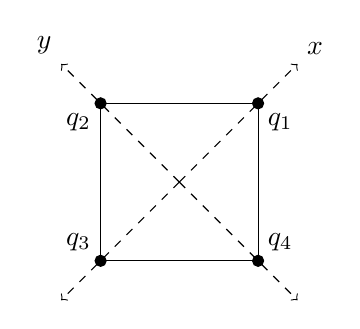
\begin{tikzpicture}
			\draw plot[mark=*,mark size = 2pt] coordinates {(0,0)(2,0)(2,2)(0,2)} -- cycle;
			\node (q) at (0,0) [above left] {$q_3$};
			\node (q) at (2,0) [above right] {$q_4$};
			\node (q) at (2,2) [below right] {$q_1$};
			\node (q) at (0,2) [below left] {$q_2$};
			\draw[dashed,->] (1,1) -- (2.5,2.5);
			\draw[dashed,->] (1,1) -- (-0.5,-0.5);
			\node (x) at (2.5, 2.5) [above right] {$x$};
			\draw[dashed,->] (1,1) -- (-0.5,2.5);
			\draw[dashed,->] (1,1) -- (2.5,-0.5);
			\node (y) at (-0.5, 2.5) [above left] {$y$};
		\end{tikzpicture}
	\end{center}
	
	Note that each charge is a distance $a / \sqrt{2}$ from the origin.  For a square rotating counter-clockwise, the locations of each of the point charges are
	\al{
		\vxq(t) &= \frac{a}{\sqrt{2}} (\cos \omg t \,\xh + \sin \omg t \,\yh), &
		\vxw(t) &= \frac{a}{\sqrt{2}} (-\sin \omg t \,\xh + \cos \omg t \,\yh), \\
		\vxe(t) &= \frac{a}{\sqrt{2}} (-\cos \omg t \,\xh - \sin \omg t \,\yh), &
		\vxr(t) &= \frac{a}{\sqrt{2}} (\sin \omg t \,\xh - \cos \omg t \,\yh).
	}
	Define the charge distributions for each of the point charges as
	\al{
		\rhoq(\vx, t) &= -q \, \delta(\vx - \vxq), &
		\rhow(\vx, t) &= q \, \delta(\vx - \vxw), &
		\rhoe(\vx, t) &= -q \, \delta(\vx - \vxe), &
		\rhor(\vx, t) &= q \, \delta(\vx - \vxr),
	}
	so the total charge distribution is
	\eq{
		\rho(\vx, t) = \sum_i \rho_i(\vx, t).
	}
	
	The quadrupole moment is defined by Wald~(2.47),
	\eq{
		\Qij = \int (3 x_i x_j - r^2 \del_{ij}) \rho \ddcx.
	}
	Note that $\Qij$ is symmetric.  Its elements are
	\al{
		Q_{11} &= \int (3 x^2 - x^2 - y^2 - z^2) [ \rhoq(\vx, t) + \rhow(\vx, t) + \rhoe(\vx, t) + \rhor(\vx, t) ] \ddcx \\
		&= q \int (2 x^2 - y^2 - z^2) [ -\delta(\vx - \vxq) + \delta(\vx - \vxw) - \delta(\vx - \vxe) + \delta(\vx - \vxr) ] \ddcx \\
		&= \frac{q a^2}{2} [ -2 \cos^2(\omg t) + \sin^2(\omg t) + 2 \sin^2(\omg t) - \cos^2(\omg t) - 2 \cos^2(\omg t) + \sin^2(\omg t) + 2 \sin^2(\omg t) - \cos^2(\omg t) ] \\
		&= 3 q a^2 [ \sin^2(\omg ) - \cos^2(\omg t) ]
		= -3 q a^2 \cos(2\omg t),
	}
	\al{
		Q_{12} & = 3 \int xy [ \rhoq(\vx, t) + \rhow(\vx, t) + \rhoe(\vx, t) + \rhor(\vx, t) ] \ddcx \\
		&= 3q \int [ -\delta(\vx - \vxq) + \delta(\vx - \vxw) - \delta(\vx - \vxe) + \delta(\vx - \vxr) ] \ddcx
		= -6 q a^2 \sin \omg t \cos \omg t
		= -3 q a^2 \sin 2\omg t \\
		&= Q_{21}, \\[2ex]
		Q_{22} &= q \int (2 y^2 - x^2 - z^2) [ -\delta(\vx - \vxq) + \delta(\vx - \vxw) - \delta(\vx - \vxe) + \delta(\vx - \vxr) ] \ddcx
		= 3 q a^2 [ \sin^2(\omg t) - \cos^2(\omg t) ] \\
		&= -Q_{11}, \\[2ex]
		Q_{13} &= Q_{23} = Q_{33} = 0.
	}
	So the quadrupole moment tensor is
	\eq{
		\ans{ Q = -3 q a^2 \mqty[
			\cos(2\omg t) & \sin(2 \omg t) & 0 \\
			\sin(2 \omg t) & -\cos(2\omg t) & 0 \\
			0 & 0 & 0
			]
			=
			\Re\!\curly{ -3 q a^2 e^{-2i \omg t} \mqty[
			1 & i & 0 \\
			i & -1 & 0 \\
			0 & 0 & 0
			] }. }
	}
	
	The magnetic induction field for quadrupole radiation is given by Jackson~(9.44),
	\eq{
		\vH = -\frac{i c k^3}{24\pi} \frac{e^{i k r}}{r} \nh \cross \vQ(\nh),
	}
	where $k$ is the wave number, $\nh$ is a unit vector in the direction of the observtion point, and the vector $\vQ(\nh)$ is defined by Jackson~(9.43) with components
	\eq{
		Q_i = \sum_j Q_{i j} n_j.
	}
	Note that $\nh = \rh$, the radial unit vector in spherical coordinates.  So in Cartesian coordinates,
	\eq{
		\nh = \sin\tht \cos\phi \,\xh + \sin\tht \sin\phi \,\yh + \cos\tht \,\zh.
	}
	Also,
	\aln{
		\Qx &= -3q a^2 \sin\tht e^{-2i \omg t} (\cos\phi + i \sin\phi)
		= -3q a^2 \sin\tht \,e^{-2i \omg t} \,e^{i\phi}, \notag \\
		\Qy &= -3q a^2 \sin\tht e^{-2i \omg t} [ i \cos\phi - \sin\phi ]
		= -3i q a^2 \sin\tht \,e^{-2i \omg t} \,e^{i \phi}, \label{Q} \\
		\Qz &= 0. \notag
	}
	Then
	\al{
		\nh \cross \vQ(\nh) &= (\ny \Qz - \nz \Qy) \,\xh + (\nz \Qx - \nx \Qz) \,\yh + (\nx \Qy - \ny \Qx) \,\zh \\
		&= -3q a^2 \sin\tht \,e^{-2i \omg t} \,e^{i \phi} [ -i \cos\tht \,\xh + \cos\tht \,\yh + \sin\tht ( i\cos\phi - \sin\phi )\,\zh \\
		&= -3q a^2 \sin\tht \,e^{-2i \omg t} \,e^{i \phi} (-i \cos\tht \,\xh + \cos\tht \,\yh + i \sin\tht \,e^{i\phi} \,\zh) \\
		&= -\frac{3}{2} q a^2 \,e^{-2i \omg t} \,e^{i \phi} \{ -i \sin(2\tht) \,\xh + \sin(2\tht) \,\yh + i [ 1 - \cos(2\tht) ] \,e^{i\phi} \,\zh \},
	}
	so
	\eq{
		\ans{ \vH = \frac{i c k^3}{16\pi} \frac{q a^2}{r} \exp[ i(kr + \phi - 2\omg t) ] \{ -i \sin(2\tht) \,\xh + \sin(2\tht) \,\yh + i [ 1 - \cos(2\tht) ] \,e^{i\phi} \,\zh \}. }
	}
	
	The electric field for quadrupole radiation is given on p.~280 in the lecture notes,
	\eq{
		\vE = \frac{i k}{\mu_0} \Zo (\nh \cross \vA) \cross \nh
		= \Zo \vH \cross \nh
		= -\frac{i c k^3}{24\pi} \Zo \frac{e^{i k r}}{r} [ \nh \cross \vQ(\nh) ] \cross \nh.
	}
	One of the vector identities on the inside cover of Jackson is
	\eq{
		\vaa \cross (\vbb \cross \vcc) = (\vaa \vdot \vcc) \vbb - (\vaa \vdot \vbb) \vcc,
	}
	so
	\eq{
		[ \nh \cross \vQ(\nh) ] \cross \nh = -\nh \cross [ \nh \cross \vQ(\nh) ]
		= \vQ(\nh) - [ \nh \vdot \vQ(\nh) ] \nh.
	}
	Note that
	\eq{
		\nh \vdot \vQ(\nh) = -3q a^2 \sin\tht \,e^{-2i \omg t} \,e^{i\phi} (\sin\tht \cos\phi + i \sin\tht \sin\phi)
		= -3q a^2 \sin^2\tht \,e^{-2i \omg t} \,e^{2i\phi}
	}
	and
	\al{
		\vQ(\nh) - [ \nh \vdot \vQ(\nh) ] \nh &= -3q a^2 \sin\tht \,e^{-2i \omg t} \,e^{i\phi} (\xh + i \,\yh) + 3q a^2 \sin^2\tht \,e^{-2i \omg t} \,e^{2i\phi} (\sin\tht \cos\phi \,\xh + \sin\tht \sin\phi \,\yh + \cos\tht \,\zh) \\
		&= 3q a^2 \sin\tht \,e^{-2i \omg t} \,e^{i\phi} [ (\sin^2\tht \cos\phi \,e^{i \phi} - 1) \,\xh + (\sin^2\tht \sin\phi \,e^{i \phi} - i) \,\yh + \sin\tht \cos\tht \,e^{i\phi} \,\zh ].
	}
	Then
	\eq{
		\ans{ \vE = -\Zo \frac{i c k^3}{8\pi} \frac{q a^2}{r} \sin\tht \,\exp[i (k r + \phi - 2\omg t)] [ (\sin^2\tht \cos\phi \,e^{i \phi} - 1) \,\xh + (\sin^2\tht \sin\phi \,e^{i \phi} - i) \,\yh + \sin\tht \cos\tht \,e^{i\phi} \,\zh ]. }
	}
	
	The angular distribution of radiation for a quadrupole is given by Jackson~(9.45),
	\eq{
		\dv{P}{\Omg} = \frac{c^2 \Zo}{1152 \pi^2} k^6 \abs{ [ \nh \cross \vQ(\nh) ] \cross \nh }^2.
	}
	According to (9.46),
	\al{
		\abs{ [ \nh \cross \vQ(\nh) ] \cross \nh }^2 &= \abs{ \vQ(\nh) }^2 - \abs{ \nh \vdot \vQ(\nh) }^2 \\
		&= \abs{ -3q a^2 \sin\tht \,e^{-2i \omg t} \,e^{i\phi} }^2 + \abs{ -3i q a^2 \sin\tht \,e^{-2i \omg t} \,e^{i\phi} }^2 - \abs{ -3q a^2 \sin^2\tht \,e^{-2i \omg t} \,e^{2i\phi} }^2 \\
		&= 9 q^2 q^4 \sin^2\tht (2 - \sin^2\tht)
		= 9 q^2 q^4 (1 - \cos^2\tht) (1 + \cos^2\tht)
		= 9 q^2 q^4 (1 - \cos^4\tht),
	}
	so
	\eq{
		\ans{ \dv{P}{\Omg} = \frac{c^2 \Zo}{128 \pi^2} k^6 q^2 q^4 (1 - \cos^4\tht). }
	}
	
	The total radiated power for a quadrupole is given by Jackson~(9.49),
	\eq{
		P = \frac{c^2 \Zo k^6}{1440 \pi} \sum_{i, j} \abs{ \Qij }^2.
	}
	Note that
	\eq{
		\sum_{i, j} \abs{ \Qij }^2 = \abs{ -3 q a^2 e^{-2i \omg t} }^2 [ 1^2 + \abs{i}^2 + \abs{i}^2 + (-1)^2 ]
		= 36 q^2 a^4,
	}
	so
	\eq{
		\ans{ P = \frac{c^2 \Zo}{40 \pi} k^6 q^2 a^4. }
	}
	
	Since $\Qij \propto e^{2i \omg t}$, \ans{the frequency of radiation is $2\omg$.}  This means $k = 2 \omg / c$.
	
	Writing the previous results in terms of the frequency, we have
	\ans{ \al{
		\vH &= \frac{i \omg^3}{2\pi c^2} \frac{q a^2}{r} \exp[ i(kr + \phi - 2\omg t) ] \{ -i \sin(2\tht) \,\xh + \sin(2\tht) \,\yh + i [ 1 - \cos(2\tht) ] \,e^{i\phi} \,\zh \}, \\[2ex]
		\vE &= -\Zo \frac{i \omg^3}{\pi c^2} \frac{q a^2}{r} \sin\tht \,\exp[i (k r + \phi - 2\omg t)] [ (\sin^2\tht \cos\phi \,e^{i \phi} - 1) \,\xh + (\sin^2\tht \sin\phi \,e^{i \phi} - i) \,\yh + \sin\tht \cos\tht \,e^{i\phi} \,\zh ],
	}
	\vfix
	\al{
		\dv{P}{\Omg} &= \frac{\Zo}{2 \pi^2 c^4} \omg^6 q^2 q^4 (1 - \cos^4\tht), &
		P &= \frac{8 \Zo}{5 \pi c^4} \omg^6 q^2 a^4.
	} }%
	\vfix
}